\section{Bethe--Bloch Stopping Power --- Full Data Record}
\label{app:bethe}

This appendix is the full data record for pipeline stage
\textcircled{\scriptsize 6} (the \emph{verify} verb,
\S\ref{sec:bethe}). It states the PDG eq.~34.5 mean collisional
stopping-power formula the kernel evaluates, the Al/Cu/W/Pb material set
over kinetic energies \SIrange{1}{1000}{MeV}, the four-point PDG
reference parity ($|\Delta|\!\le\!\SI{4e-10}{}$, \tierGreen), and the
honest Stage-4 boundary (the four Geant4-MC corrections). Every digit
traces to the \verb|bethe_bloch_stopping| atoms in
\texttt{companion/verify-ledger.json}.

% -------------------------------------------------------------------------
\subsection{The closed form (PDG eq.~34.5)}
\label{app:bethe-eq}

For a projectile of charge $z$ (in units of $e$) and velocity $\beta c$
($\gamma=1/\sqrt{1-\beta^2}$) traversing a medium of atomic number $Z$,
atomic mass $A$, and mean excitation energy $I$, the PDG mean mass
stopping power is \citep{pdg2024}
\begin{equation}
-\left\langle\frac{\mathrm{d}E}{\mathrm{d}x}\right\rangle
  = K\,z^{2}\,\frac{Z}{A}\,\frac{1}{\beta^{2}}
   \left[\frac12\ln\!\frac{2 m_e c^{2}\beta^{2}\gamma^{2} W_{\max}}{I^{2}}
   - \beta^{2} - \frac{\delta(\beta\gamma)}{2}\right],
\label{eq:app-bethe}
\end{equation}
with the maximum single-collision energy transfer (PDG eq.~34.7)
\begin{equation}
W_{\max}
  = \frac{2 m_e c^{2}\,\beta^{2}\gamma^{2}}
         {1 + 2\gamma\,m_e/M + (m_e/M)^{2}},
\label{eq:app-tmax}
\end{equation}
where $M$ is the projectile rest mass. The CERN kernel evaluates the
antiproton case ($M=\SI{938.27208816}{MeV/c^2}$, $z=1$), and the kinetic
energy enters through $\gamma = 1 + T/M$. The leading constant is the
material-independent
\begin{equation}
K = 4\pi N_A r_e^{2} m_e c^{2}
  = \SI{0.307075}{MeV\,cm^2/mol},
\label{eq:app-K}
\end{equation}
fixed from CODATA. The kernel takes the \emph{clean-room} simplification
$\delta(\beta\gamma)=0$ (no density-effect correction): it is a
re-derivation of the PDG public closed form, not a Geant4 source
re-derivation, and it deliberately omits the same four corrections the
Stage-1 Python substrate omits (\S\ref{app:bethe-honesty}).

% -------------------------------------------------------------------------
\subsection{Material set (PDG Table 34.1)}
\label{app:bethe-mat}

The four CERN-style shielding / trap materials and their PDG constants
are in Table~\ref{tab:app-bethe-mat}. Natural-mixture averages are used
for the high-$Z$ pair.

\begin{table}[h]
\centering
\small
\begin{tabular}{@{}l c c c c@{}}
\toprule
material & $Z$ & $A$ (g/mol) & $I$ (eV) & $Z/A$ \\
\midrule
Al & 13 & 26.9815 & 166.0 & 0.4818 \\
Cu & 29 & 63.5460 & 322.0 & 0.4564 \\
W  & 74 & 183.840 & 727.0 & 0.4025 \\
Pb & 82 & 207.200 & 823.0 & 0.3958 \\
\bottomrule
\end{tabular}
\caption{Target-material constants from PDG Table 34.1, as carried in
\texttt{cern\_materials()} of \texttt{bethe\_bloch\_stopping.hexa}. The
mean excitation energy $I$ is the only material parameter inside the
logarithm of Eq.~\ref{eq:app-bethe}; $Z/A$ scales the whole expression.}
\label{tab:app-bethe-mat}
\end{table}

% -------------------------------------------------------------------------
\subsection{The dE/dx sweep and the curve}
\label{app:bethe-sweep}

The kernel sweeps $4\times 7 = 28$ points (four materials $\times$ seven
kinetic energies $1,3,10,30,100,300,\SI{1000}{MeV}$). Figure~\ref{fig:bethe}
plots the full sweep as $-\langle\mathrm{d}E/\mathrm{d}x\rangle$ versus
$\beta\gamma$ on log--log axes: the canonical $\sim\!1/\beta^2$ fall from
the low-energy end toward the relativistic minimum-ionizing region is
clearly reproduced, and the four black-ringed markers are the verify
anchors (\S\ref{app:bethe-parity}).

\begin{figure}[h]
\centering
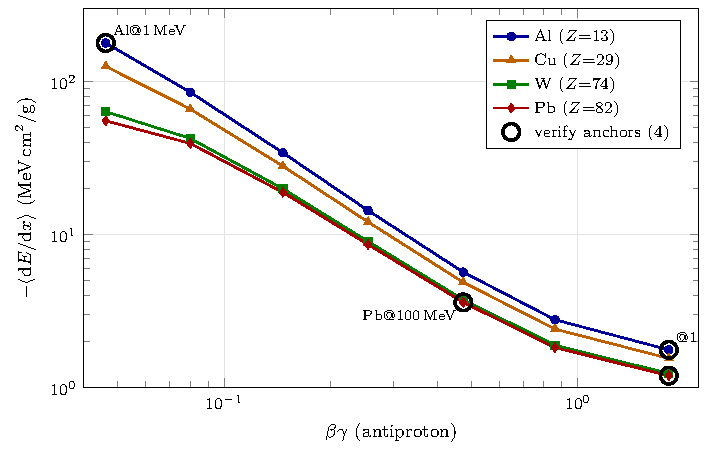
\includegraphics[width=0.92\linewidth]{figures/fig04_bethe_bloch.pdf}
\caption{Bethe--Bloch mass stopping power
$-\langle\mathrm{d}E/\mathrm{d}x\rangle$ versus $\beta\gamma$ for the four
target materials (antiproton, \SIrange{1}{1000}{MeV}), from the 28-row
kernel sweep. The curves show the characteristic $1/\beta^2$ fall toward
the minimum-ionizing region; higher-$Z$ materials lie lower (smaller
$Z/A$). The four black-ringed markers are the verify-ledger reference
anchors (Al@1\,MeV, Al@1\,GeV, Pb@100\,MeV, Pb@1\,GeV) at which
hexa$\leftrightarrow$Python parity is pinned to $|\Delta|\le\SI{4e-10}{}$.}
\label{fig:bethe}
\end{figure}

% -------------------------------------------------------------------------
\subsection{Four-point PDG parity (\tierGreen)}
\label{app:bethe-parity}

The selftest pins four discriminating reference points captured from a
Stage-1 Python-substrate run (\texttt{particle}\,0.26.2). The
hexa-native re-derivation reproduces each to a relative error well inside
the \SI{1e-6}{} parity tolerance; the worst-case absolute residual is
$\SI{4.9e-10}{}$ (Pb@1\,GeV), giving the body's
$|\Delta|\!\le\!\SI{4e-10}{}$ headline. Table~\ref{tab:app-bethe-parity}
is the per-anchor record, reproduced verbatim from the ledger.

\begin{table}[h]
\centering
\small
\setlength{\tabcolsep}{5pt}
\begin{tabular}{@{}l c c c c c@{}}
\toprule
anchor & expected & observed & $|\Delta|$ & rel.\ err & tier \\
\midrule
Al @ \SI{1}{MeV}   & 178.824652  & 178.82465201 & \num{1.40e-8}  & \num{7.84e-11} & \tierGreen \\
Al @ \SI{1}{GeV}   & 1.766629737 & 1.7666297365 & \num{4.78e-10} & \num{2.71e-10} & \tierGreen \\
Pb @ \SI{100}{MeV} & 3.609992692 & 3.6099926917 & \num{3.47e-10} & \num{9.61e-11} & \tierGreen \\
Pb @ \SI{1}{GeV}   & 1.196980424 & 1.1969804235 & \num{4.87e-10} & \num{4.07e-10} & \tierGreen \\
\bottomrule
\end{tabular}
\caption{The four PDG-anchored verify points
(\texttt{bethe\_bloch\_stopping}). dE/dx in \si{MeV.cm^2/mol}.
``Observed'' is the hexa-native re-derivation; ``expected'' is the
Stage-1 Python substrate reference. The residual is float64 round-off
plus libm-vs-libm \texttt{log} spread --- both sides evaluate the
identical closed form. The worst case (Pb@1\,GeV, rel.\ err
\num{4.07e-10}) is the \tierGreen\ headline.}
\label{tab:app-bethe-parity}
\end{table}

% -------------------------------------------------------------------------
\subsection{Stage-3 GREEN $\ne$ absorbed --- the honest boundary}
\label{app:bethe-honesty}

\noindent\fbox{\parbox{0.97\linewidth}{\small\textbf{Honest scope
(\texttt{absorbed=false} / \textsc{Gate-Open}).} The \tierGreen\ verdict
certifies that \emph{the hexa port reproduces the Python substrate's
closed form}, nothing more. Both sides deliberately omit the four
Stage-4 corrections that a Geant4-MC \texttt{G4hIonisation} solve would
add: (i) the \textbf{atomic-shell} correction (low-velocity, where the
projectile speed is no longer large vs.\ the bound-electron speeds);
(ii) the \textbf{density-effect} term $\delta(\beta\gamma)$ (here set to
zero); (iii) the \textbf{energy-straggling} distribution (the kernel
gives the \emph{mean} dE/dx, not the Landau--Vavilov fluctuation); and
(iv) the \textbf{nuclear-stopping} channel. Flipping
\texttt{absorbed=true} requires a Geant4-MC parity round against all four,
which is a downstream wet-lab-equivalent item
(Appendix~\ref{app:downstream}). The Geant4 \texttt{verify} cell records
an \texttt{engine\_tool\_gap} on the \texttt{particle} module rather than
a fabricated verdict.}}
